%
%  Wakefield Acceleration
% ========================
%

\chapter{The AWAKE Experiment}
\label{Ch:WFA}

AWAKE is the first proton driven wakefield accelerator experiment in the world.
It is a proof-of-concept experiment aiming to inform a design for future high energy accelerators~\cite{gschwendtner:2016} and to prove the feasibility of such an accelerator.
The proton drive beam for the experiment is delivered by the Super Proton Synchrotron (SPS) at CERN at an energy of $400\unit{GeV}$, and joined by an electron witness beam in a $10\unit{m}$ plasma stage.

AWAKE is physically located at the former site of the CERN Neutrinos to Gran Sasso experiment (CNGS) \cite{gschwendtner:2010} in a tunnel below the Swiss-French border, and is connected to the SPS at SPS Point 4.
The connection of the AWAKE experiment to the rest of the CERN accelerator complex is illustrated in Fig.~\ref{Fig:WFA:AccComp}.

\begin{figure}[hbt]
    \centering
    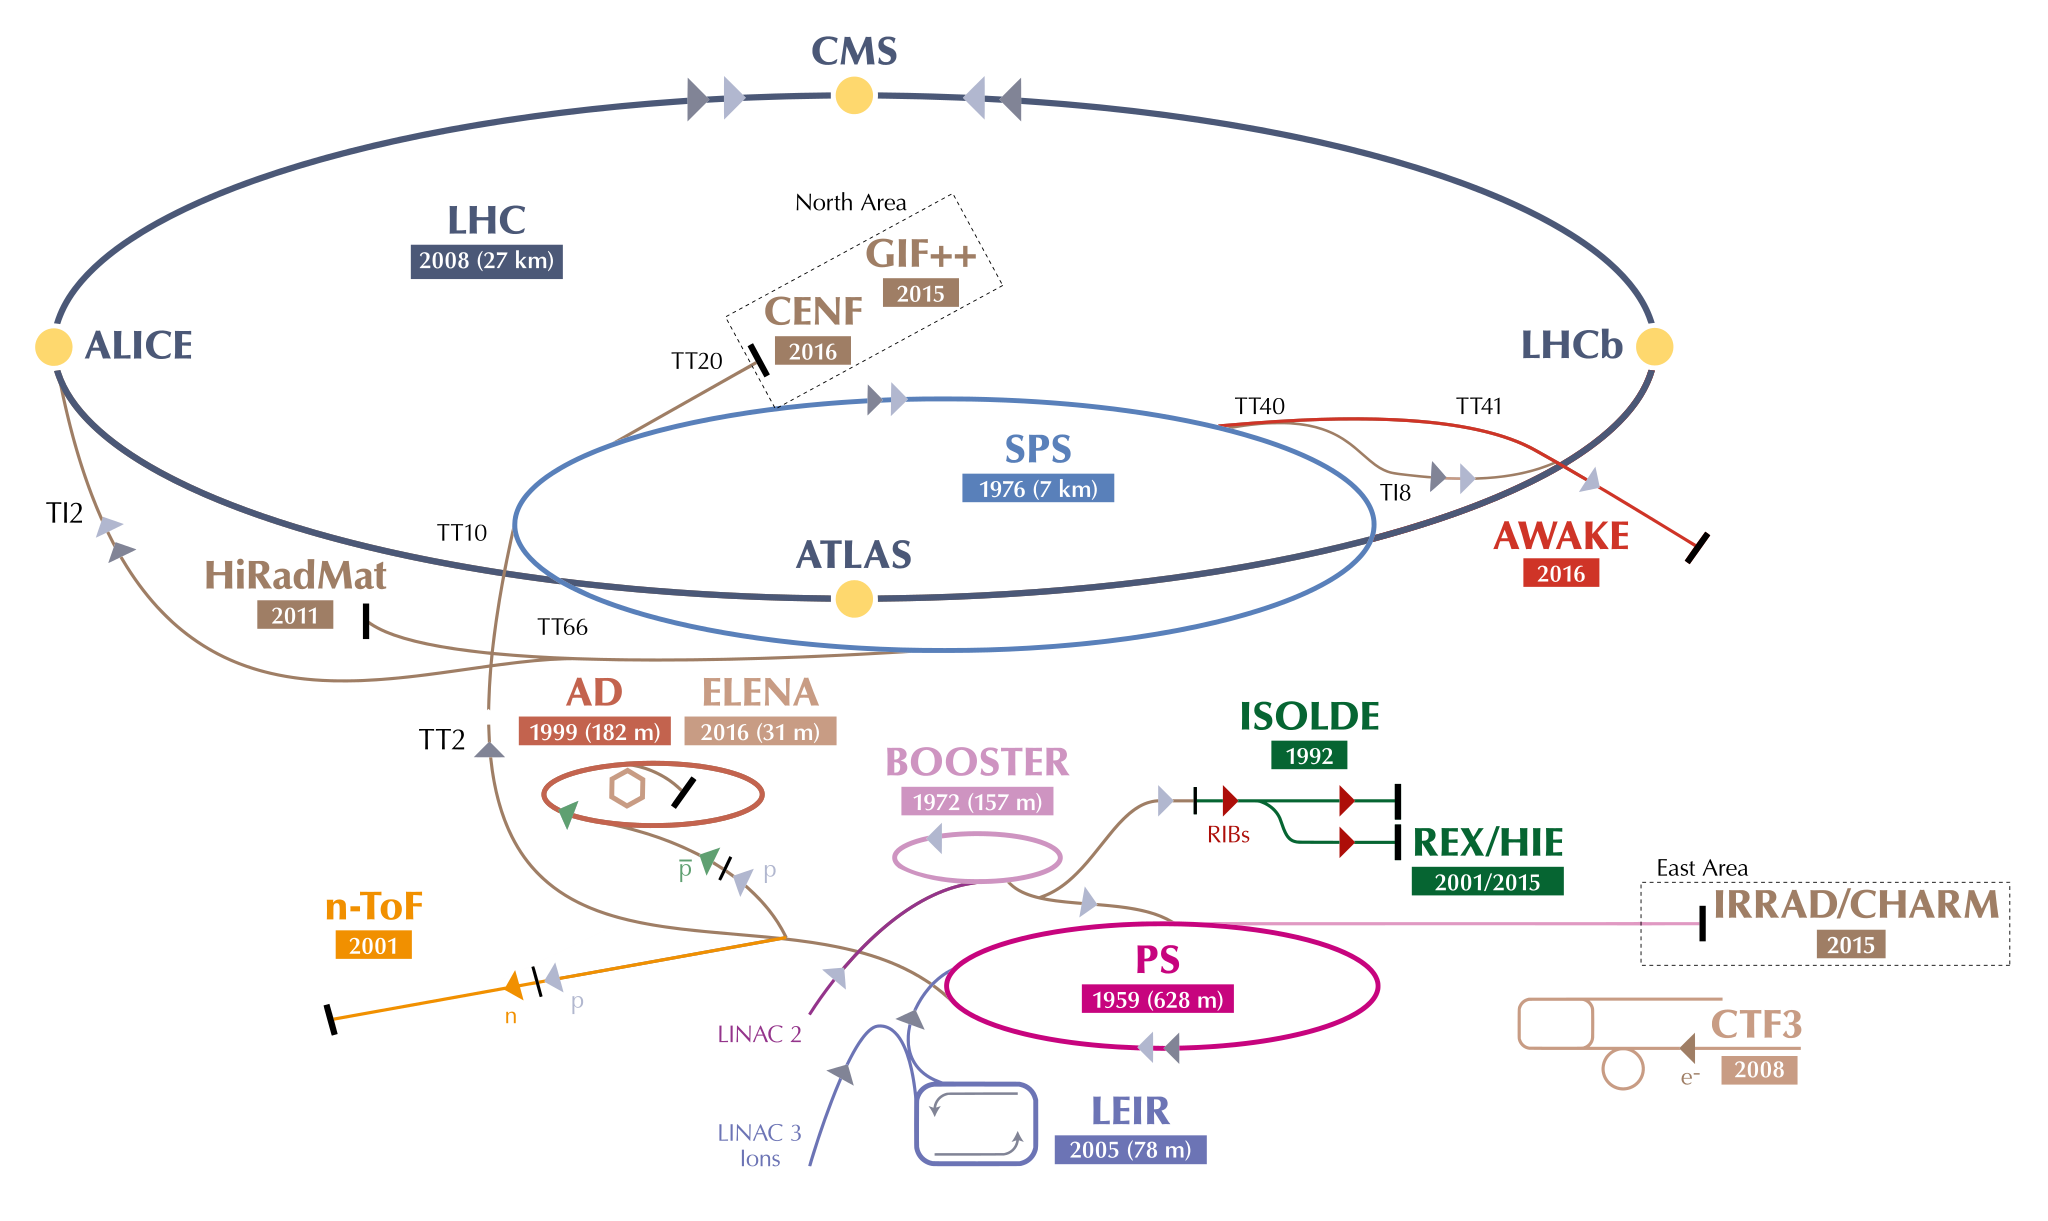
\includegraphics[width=0.99\linewidth,trim={20mm 0mm 20mm 0mm},clip]{figures/AcceleratorComplex}
    \caption{\label{Fig:WFA:AccComp}
        An overview of the CERN Accelerator Complex \cite{add:mobs:2016}.
    }
\end{figure}

% ================================================================================================================================ %
\section{Evolution of the Concept}
\label{WFA:History}

While AWAKE is the first proton driven wakefield experiment, a number of experiments with electron drive beams have confirmed the models produced by theory and simulations.
The first experimental results of plasma wakefield acceleration were conducted at the Advanced Accelerator Test Facility at Argonne National Laboratory (ANL) outside Chicago, USA, and published in 1988~\cite{rosenzweig:1988}.
The experiment split an electron beam of a few $\unit{nC}$ into a drive and a witness beam, and demonstrated that the drive beam generates accelerating wakefields as well as strong transverse fields. The accelerating gradient they produced was modest, only a few $\unit{MeV}$.

More recently, $\unit{GeV}$ level acceleration gradients have been achieved with an electron bunch at SLAC, where parts of a $42\unit{GeV}$ electron bunch saw energy doubling in an $85\unit{cm}$ plasma cell.
The results were published in Nature in 2007~\cite{blumenfeld:2007}. The plasma stage produced a continuous spread in energy up to about $85\unit{GeV}$.
However, only a small fraction of the charge was accelerated to these energies.
An experiment at SLAC later produced a discrete, accelerated bunch with a core of $74\unit{pC}$ in an accelerating gradient of $4.4\unit{GeV/m}$~\cite{litos:2014}.

%Self modulation at FACET \cite{adli:2016}
%Review by Patric \cite{muggli:2009}

% ================================================================================================================================ %
\section{AWAKE: A Design Overview}
\label{WFA:Design}

AWAKE is, as of the writing of this thesis, operational and in Run~1.
The proton beam line arriving from the SPS joins with the laser beam and the electron beam line, and connects to a $10\unit{m}$ plasma stage at the end of the tunnel.
In addition, an electron source has been installed, and a new side tunnel had to be dug to fit the electron beam line connecting the source to the main assembly.
Figure \ref{Fig:WFA:AWAKE} gives and overview of the experimental layout in the tunnel.
The old CNGS target is still present behind a shielding wall, as it is highly radioactive.
This, unfortunately, has created some constraints for fitting the downstream beam line and diagnostics, and may pose additional challenges for Run~2 if longer or multiple plasma stages are needed.

\begin{figure}[hbt]
    \centering
    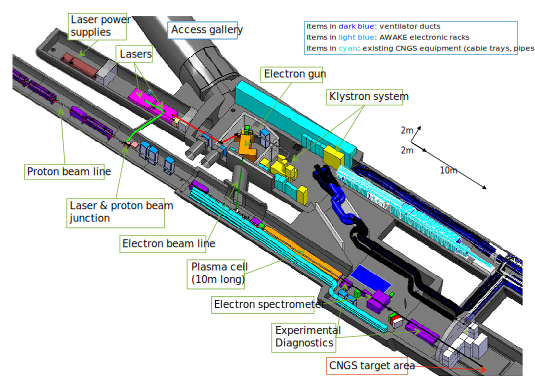
\includegraphics[width=0.99\linewidth,trim={0mm 0mm 0mm 0mm},clip]{figures/AwakeExperiment}
    \caption{\label{Fig:WFA:AWAKE}
        Drawing of the AWAKE experimental area with the key components labelled.
    }
\end{figure}

% ================================================================================================================================ %
\subsection{Plasma Source}
\label{WFA:Design:Plasma}

The requirements for the plasma source for AWAKE Run~1 were a $10\unit{m}$ long cell capable of a plasma electron density ranging from $1-10\nexp{14}\unit{cm}^{-3}$.
The density variation should be within $0.2\%$, and the radius of the plasma channel should be $\geq 1\unit{mm}$.
The plasma should also consist of heavy ions to mitigate ion motion~\cite{caldwell:2015}.

\begin{figure}[hbt]
    \centering
    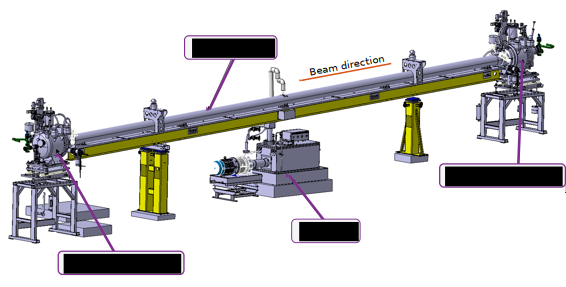
\includegraphics[width=0.99\linewidth,trim={0mm 0mm 0mm 0mm},clip]{figures/PlasmaCell}
    \caption{\label{Fig:WFA:PlasmaCell}
        Drawing of the plasma stage and its related components, as presented in the 2016 AWAKE Status Report~\cite{awake_collaboration:2016}.
    }
\end{figure}

For the AWAKE vapour source, rubidium (Rb) was chosen.
Rubidium has a low melting point, $39.3\celsius$; a low first ionisation energy, $4.18\unit{eV}$; and a standard atomic weight of $85.47$.
The plasma wavelength of rubidium ions with a $+1$ charge is roughly $400$ times that of the plasma electrons (see Equation~\ref{EQ:PWFA:L0W0}), preventing significant ion motion for AWAKE application~\cite{vieira:2012a}.
An additional benefit of using an alkaline metal like rubidium is that the second ionisation level is significantly higher, $27.3\unit{eV}$, making it relatively easy to prevent further ionisation and thus a lower charge/mass ratio~\cite{awake_collaboration:2017}.
The rubidium vapour is created by heating the reservoir and the plasma cell to around $150-230\celsius$ to reach the density range required for AWAKE~\cite{caldwell:2015,muggli:2017a}.

The ionisation of the Rb vapour is achieved with a short laser pulse co-propagating with the proton drive beam.
The laser can be timed such that the plasma channel is created inside the beam itself.
The short laser pulse produces a sharp plasma edge that provides a good seed for the self-modulation instability~\cite{vieira:2014a}, as discussed in Section~\ref{Int:DBeam:SMI}.
The section of the proton beam ahead of the laser does not interact strongly with the neutral rubidium vapour, although a low level of impact ionisation does occur.
However, this effect is not significant~\cite{awake_collaboration:2017}.

The ionisation laser used for AWAKE is a $780\unit{nm}$ Ti:Sapphire laser with a pulse length of $120\unit{fs}$ and a maximum compressed energy of $450\unit{mJ}$.
The peak intensity is around $1.2\nexp{14}\unit{W/cm}^{2}$, with a spot size radius of $1\unit{mm}$~\cite{awake_collaboration:2017}.
The appearance intensity needed for ionisation of rubidium is around $1.7\nexp{12}\unit{W/cm}^{2}$~\cite{augst:1989}.
Ionisation of a second electron requires some $455$ times higher intensity, so secondary ionisation is not expected~\cite{muggli:2017a}.

The plasma density produced by the laser pulse is currently measured with a Mach-Zehnder type interferometers, which produces an interferogram that requires further processing to provide a density measurement \cite{oz:2016}.
There are also possible solutions proposed for real-time diagnostics using a Michelson-type interferometer \cite{djotyan:2018}.

% ================================================================================================================================ %
\subsection{Electron Source}
\label{WFA:Design:ESource}

The AWAKE electron source for Run~1 consists of a $2.5$ cell RF-gun and a $1\unit{m}$ long booster structure, both operating at $3\unit{GHz}$, a cathode transfer chamber, beam diagnostics, and a beam transport line connecting it to the proton beam line.
The beam is boosted to up to $20\unit{MeV}$ by a constant gradient acceleration structure.
The RF-gun and the booster are powered by a $30\unit{MW}$ klystron~\cite{awake_collaboration:2017,pepitone:2016}.
Several of the components, including the RF-gun and klystron, were re-purposed from the former PHIN injector in the CLIC test facility~\cite{chevallay:2012}.
An overview of the electron source and the accelerating structure can be seen in Figure~\ref{Fig:WFA:ESource}.

\begin{figure}[hbt]
    \centering
    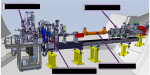
\includegraphics[width=0.70\linewidth,trim={0mm 0mm 0mm 0mm},clip]{figures/ElectronSource}
    \caption{\label{Fig:WFA:ESource}
        Drawing of the electron source and accelerating structure~\cite{pepitone:2016}.
    }
\end{figure}

% ================================================================================================================================ %
\section{Stages of the Experiment}
\label{WFA:AWAKE}

All stages of the AWAKE experiment has been studied in detail in simulations.
Due to the large number of parameters for the plasma and laser, and the drive and witness beams, the range of interest of these have both been determined by previous experiments and AWAKE specific simulations.

\begin{table}[hbt]
    \centering
    \caption{\label{T:AWAKERuns}
        Nominal AWAKE beam parameters for Run~1~\cite{gschwendtner:2014, gschwendtner:2016} and Run~2~\cite{adli:2016a}.
    }
    \begin{tabular}{p{57mm}p{20mm}p{20mm}p{28mm}}
        \rowcolor{tblhead}
        \texthh{Experiment}                   & \texthh{Protons}  & \multicolumn{2}{l}{\texthh{Electrons}}        \\
        \rowcolor{tblunit}
        \texthh{Parameters}                   & \texthu{Run 1\&2} & \texthu{Run 1}    & \texthu{Run 2}            \\
        \hline
        Momentum                              & $400\unit{GeV}$   & $16\unit{MeV}$    & $\gtrsim 50\unit{MeV}$    \\
        Charge                                & $4.8\unit{nC}$    & $200\unit{pC}$    & $67-200\unit{pC}$         \\
        Particles                             & $3\nexp{11}$      & $1.25\nexp{9}$    & $0.42-1.25\nexp{9}$       \\
        Bunch length ($\sigma_{z}$)           & $12\unit{cm}$     & $1.2\unit{mm}$    & $40-60\unit{\mu m}$       \\
        Bunch size ($\sigma_{x,y}$)           & $200\unit{\mu m}$ & $250\unit{\mu m}$ & \textemdash               \\
        Normalised emittance ($\emitN$)       & $3.5\unit{\mu m}$ & $2\unit{\mu m}$   & $\lesssim 10\unit{\mu m}$ \\
        Relative energy spread ($\Delta p/p$) & $0.035\%$         & $0.5\%$           & $\mathrm{few}\,\%$        \\
        Beta function ($\beta^{*}_{x,y}$)     & $4.9\unit{m}$     & $0.4\unit{m}$     & \textemdash               \\
        Dispersion ($D^{*}_{x,y}$)            & $0$               & $0$               & \textemdash               \\
        \hline
    \end{tabular}
\end{table}

The key, nominal parameters for Run~1, and the planned parameters for Run~2, are listed in Table~\ref{T:AWAKERuns}.

% ================================================================================================================================ %
\subsection{AWAKE Run 1}
\label{WFA:AWAKE:R1}

The primary focus of Run~1 of AWAKE was to study the wakefields generated by the SPS proton beam in the $10\unit{m}$ Rubidium plasma stage.
In the first phase the main focus was on measuring the self-modulation instability and the frequency of this modulation in relation to the plasma density.
The second phase aims to sample the generated wakefields with a long electron beam capable of sampling a full plasma wavelength~\cite{adli:2016a}.

A large part of the work involved in Run~1 is related to the operation and diagnostics of all the essential elements involved in the experiment, from the vapour cell and the laser system, to the beam transport; and their respective diagnostics systems.
Especially the size and and density uniformity of the plasma channel are essential parameters to control.

% ================================================================================================================================ %
\subsubsection{The Self-Modulation Instability in AWAKE}
\label{WFA:SMI}

Run~1 of AWAKE has confirmed that seeded self-modulation of an SPS proton bunch indeed does occur in the AWAKE vapour stage when the laser is operating at high power.
The results shown in Figure~\ref{Fig:SMI:Results} were presented in the thesis work of M.~Turner for the AWAKE experiment~\cite{turner:2017}.
The left-most figure shows that no modulation occurs when the laser is at a low power setting and no plasma produced.
When the laser is switched to high power in the middle figure, the SPS bunch is defocused starting from the region where the laser is positioned.
The time scale of the vertical axis is too large to show if self-modulation does occur, but the right-most figure shows a region of the defocused bunch at a higher resolution, where the micro-bunch structure is clearly visible.

\begin{figure}[hbt]
    \centering
    \includegraphics[width=0.90\linewidth,trim={0mm 0mm 0mm 0mm},clip]{figures/SMI-Turner}
    \caption{\label{Fig:SMI:Results}
        Resolved streak camera images of the SPS proton beam propagating through the Rb vapour in the AWAKE experiment.
        The read lines indicate the region of the laser pulse.
        \textbf{Left:} The laser on low power; that is, no plasma.
        \textbf{Centre:} The laser on high power, ionising the vapour and defocusing the beam.
        \textbf{Right:} A high resolution image of the defocused region, showing beam modulation.
        The image is borrowed from the thesis of M. Turner~\cite{turner:2017}.
    }
\end{figure}

% ================================================================================================================================ %
\subsection{AWAKE Run 2}
\label{WFA:AWAKE:R2}

The electron bunch for Run~1 was designed to sample all phases of the accelerating field, and is therefore both long with respect to the optimal phase of the field (see Section~\ref{Int:BPI:BLoad}), and wide compared to the matching condition with the plasma density (see Equation~\ref{EQ:BMatch}).
It is expected that for Run~1, only a small section of electron bunch will be accelerated, and energy spread and emittance will be large, but it will give a good impression of the performance of the different regions of the accelerating structure generated by the SPS drive bunch.
This step is necessary to verify simulation results, and will help determine the experimental set-up for the next stage of AWAKE, Run~2.

The first target objective of Run~2 is the successful acceleration of a short electron beam, looking to maximise energy and charge while retaining a low emittance and energy spread in order to demonstrate that it is indeed possible to produce an accelerated beam with sufficient quality for further experimental applications.
The results from Run~1 and simulations will dictate the parameters of the Run~2 electron bunch in order to achieve these goals.

The second target of Run~2 is to demonstrate scalability.
Previous experiments have shown that high accelerating gradients can be achieved in short plasma stages, but using lasers or electron bunches as drivers puts constraints on the distances such gradients can be sustained over (see Section~\ref{Int:BPI}).
As previously discussed, proton drive beams can propagate significantly longer in plasma, sustaining large accelerating fields over very long distances.
However, producing long plasma channels with high enough quality to sustain such an accelerating structure may prove to be challenging.
The Rubidium plasma stage currently uses a laser to ionise the vapour.
How far the laser can propagate, as well as the availability of high power lasers, puts limits on how long such a plasma channel can be.

% Reshuffle the below
There are two main options for Run~2 to get around the challenge of long plasma stages.
\begin{enumerate}
    \item Use two stages, where the first stage is used to let the proton bunch undergo self-modulation, and a second plasma stage that is used in its entirety for acceleration.
    In this scenario, the electron bunch will be injected between the two stages.
    However, the optics required to steer the electron bunch onto the axis of the proton bunch implies a gap between these two stages would be required.
    Such a gap has a negative effect on the amplitude of the longitudinal field, reducing the maximum possible gradient for the second stage.
    This issue is in particular covered in Section~12 of the 2016 AWAKE Status Report \cite{awake_collaboration:2016}.
    An additional limitation to this solution is that the AWAKE experimental area itself has limited space for extending beam lines and adding multiple plasma stages.
    This is due to the highly radioactive target and shielding from the CNGS experiment is still present, and in the way of expanding the area \cite{adli:2016a}.
    \item To avoid the problems with staging, the ideal option would be to use a single plasma stage.
    This would require a different approach to the plasma source.
    Such alternatives are currently being looked into.
\end{enumerate}

The simulation work presented in Chapters~\ref{Ch:SimS} and~\ref{Ch:SimA} in this thesis assumes option~1, in that the simulations assume that the available wakefield is reduced due to a gap between the two stages.

% ================================================================================================================================ %
